\documentclass{standalone}
\usepackage{tikz}
\usetikzlibrary{patterns, positioning}


\begin{document}
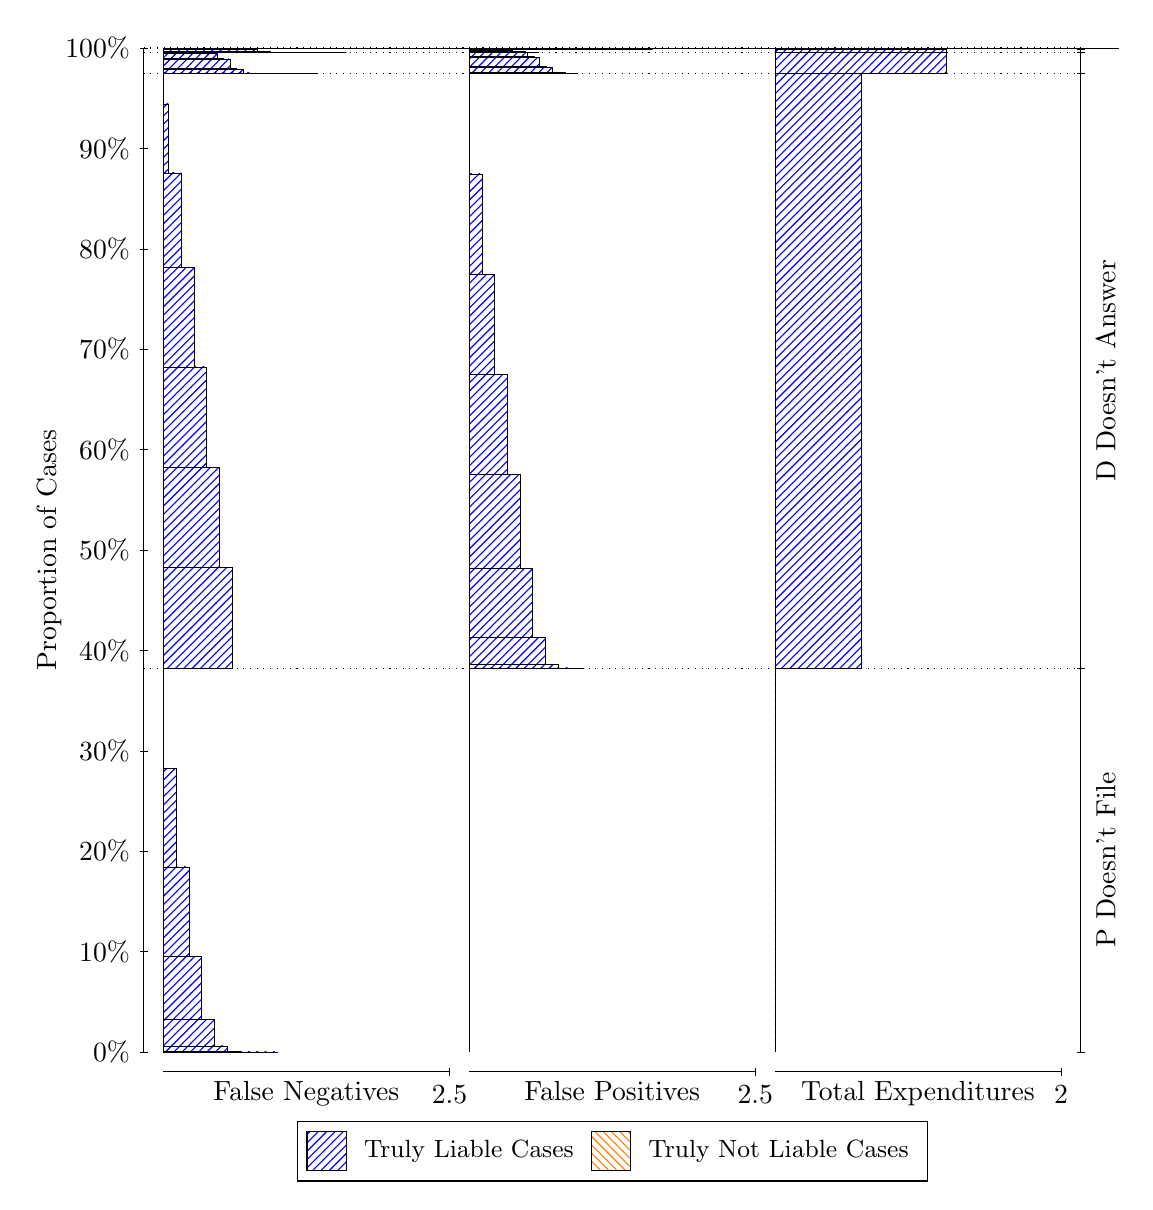
\begin{tikzpicture}
\draw[black, very thin] (1.5,1.75) -- (1.5,14.5);
\node[rotate=90, text=black, anchor=center] at (0.3, 8.125) {Proportion of Cases};
\draw[black, very thin] (1.45,1.75) -- (1.55,1.75);
\node[text=black, anchor=east] at (1.45, 1.75) {0\%};
\draw[black, very thin] (1.45,3.025) -- (1.55,3.025);
\node[text=black, anchor=east] at (1.45, 3.025) {10\%};
\draw[black, very thin] (1.45,4.3) -- (1.55,4.3);
\node[text=black, anchor=east] at (1.45, 4.3) {20\%};
\draw[black, very thin] (1.45,5.575) -- (1.55,5.575);
\node[text=black, anchor=east] at (1.45, 5.575) {30\%};
\draw[black, very thin] (1.45,6.85) -- (1.55,6.85);
\node[text=black, anchor=east] at (1.45, 6.85) {40\%};
\draw[black, very thin] (1.45,8.125) -- (1.55,8.125);
\node[text=black, anchor=east] at (1.45, 8.125) {50\%};
\draw[black, very thin] (1.45,9.4) -- (1.55,9.4);
\node[text=black, anchor=east] at (1.45, 9.4) {60\%};
\draw[black, very thin] (1.45,10.675) -- (1.55,10.675);
\node[text=black, anchor=east] at (1.45, 10.675) {70\%};
\draw[black, very thin] (1.45,11.95) -- (1.55,11.95);
\node[text=black, anchor=east] at (1.45, 11.95) {80\%};
\draw[black, very thin] (1.45,13.225) -- (1.55,13.225);
\node[text=black, anchor=east] at (1.45, 13.225) {90\%};
\draw[black, very thin] (1.45,14.5) -- (1.55,14.5);
\node[text=black, anchor=east] at (1.45, 14.5) {100\%};

\draw[black, very thin] (13.4,1.75) -- (13.4,14.5);
\draw[black, very thin] (13.35,1.75) -- (13.45,1.75);
\node[anchor=west] at (13.35, 1.75) {};
\draw[black, very thin] (13.35,6.6251) -- (13.45,6.6251);
\node[anchor=west] at (13.35, 6.6251) {};
\draw[black, very thin] (13.35,14.178) -- (13.45,14.178);
\node[anchor=west] at (13.35, 14.178) {};
\draw[black, very thin] (13.35,14.447) -- (13.45,14.447);
\node[anchor=west] at (13.35, 14.447) {};
\draw[black, very thin] (13.35,14.49) -- (13.45,14.49);
\node[anchor=west] at (13.35, 14.49) {};
\draw[black, very thin] (13.35,14.5) -- (13.45,14.5);
\node[anchor=west] at (13.35, 14.5) {};
\draw[black, very thin] (13.35,14.5) -- (13.45,14.5);
\node[anchor=west] at (13.35, 14.5) {};

\draw[black, very thin, pattern color=blue, pattern=north east lines] (1.75,1.75) rectangle (3.2033,1.75);
\draw[black, very thin, pattern color=blue, pattern=north east lines] (1.75,1.75) rectangle (3.0419,1.75);
\draw[black, very thin, pattern color=blue, pattern=north east lines] (1.75,1.75) rectangle (2.8804,1.7503);
\draw[black, very thin, pattern color=blue, pattern=north east lines] (1.75,1.7503) rectangle (2.7189,1.7569);
\draw[black, very thin, pattern color=blue, pattern=north east lines] (1.75,1.7569) rectangle (2.5574,1.8286);
\draw[black, very thin, pattern color=blue, pattern=north east lines] (1.75,1.8286) rectangle (2.3959,2.1684);
\draw[black, very thin, pattern color=blue, pattern=north east lines] (1.75,2.1684) rectangle (2.2344,2.965);
\draw[black, very thin, pattern color=blue, pattern=north east lines] (1.75,2.965) rectangle (2.073,4.1004);
\draw[black, very thin, pattern color=blue, pattern=north east lines] (1.75,4.1004) rectangle (1.9115,5.3525);
\draw[black, very thin, pattern color=orange, pattern=north west lines] (1.75,5.3525) rectangle (1.75,5.3525);
\draw[black, very thin, pattern color=blue, pattern=north east lines] (1.75,5.3525) rectangle (1.75,6.6251);
\draw[black, very thin, pattern color=blue, pattern=north east lines] (1.75,6.6251) rectangle (2.622,7.9002);
\draw[black, very thin, pattern color=blue, pattern=north east lines] (1.75,7.9002) rectangle (2.4605,9.1752);
\draw[black, very thin, pattern color=blue, pattern=north east lines] (1.75,9.1752) rectangle (2.299,10.45);
\draw[black, very thin, pattern color=blue, pattern=north east lines] (1.75,10.45) rectangle (2.1376,11.718);
\draw[black, very thin, pattern color=blue, pattern=north east lines] (1.75,11.718) rectangle (1.9761,12.914);
\draw[black, very thin, pattern color=blue, pattern=north east lines] (1.75,12.914) rectangle (1.8146,13.791);
\draw[black, very thin, pattern color=orange, pattern=north west lines] (1.75,13.791) rectangle (1.75,13.791);
\draw[black, very thin, pattern color=blue, pattern=north east lines] (1.75,13.791) rectangle (1.75,14.178);
\draw[black, very thin, pattern color=blue, pattern=north east lines] (1.75,14.178) rectangle (3.712,14.178);
\draw[black, very thin, pattern color=blue, pattern=north east lines] (1.75,14.178) rectangle (3.6393,14.178);
\draw[black, very thin, pattern color=blue, pattern=north east lines] (1.75,14.178) rectangle (3.5667,14.178);
\draw[black, very thin, pattern color=blue, pattern=north east lines] (1.75,14.178) rectangle (3.5505,14.178);
\draw[black, very thin, pattern color=blue, pattern=north east lines] (1.75,14.178) rectangle (3.4779,14.178);
\draw[black, very thin, pattern color=blue, pattern=north east lines] (1.75,14.178) rectangle (3.4052,14.178);
\draw[black, very thin, pattern color=blue, pattern=north east lines] (1.75,14.178) rectangle (3.389,14.178);
\draw[black, very thin, pattern color=blue, pattern=north east lines] (1.75,14.178) rectangle (3.3164,14.178);
\draw[black, very thin, pattern color=blue, pattern=north east lines] (1.75,14.178) rectangle (3.2437,14.178);
\draw[black, very thin, pattern color=blue, pattern=north east lines] (1.75,14.178) rectangle (3.2276,14.178);
\draw[black, very thin, pattern color=blue, pattern=north east lines] (1.75,14.178) rectangle (3.1549,14.178);
\draw[black, very thin, pattern color=blue, pattern=north east lines] (1.75,14.178) rectangle (3.0822,14.178);
\draw[black, very thin, pattern color=blue, pattern=north east lines] (1.75,14.178) rectangle (3.0661,14.178);
\draw[black, very thin, pattern color=blue, pattern=north east lines] (1.75,14.178) rectangle (2.9934,14.178);
\draw[black, very thin, pattern color=blue, pattern=north east lines] (1.75,14.178) rectangle (2.9207,14.183);
\draw[black, very thin, pattern color=blue, pattern=north east lines] (1.75,14.183) rectangle (2.9046,14.183);
\draw[black, very thin, pattern color=blue, pattern=north east lines] (1.75,14.183) rectangle (2.8319,14.183);
\draw[black, very thin, pattern color=blue, pattern=north east lines] (1.75,14.183) rectangle (2.7593,14.234);
\draw[black, very thin, pattern color=blue, pattern=north east lines] (1.75,14.234) rectangle (2.7431,14.234);
\draw[black, very thin, pattern color=blue, pattern=north east lines] (1.75,14.234) rectangle (2.6704,14.239);
\draw[black, very thin, pattern color=blue, pattern=north east lines] (1.75,14.239) rectangle (2.5978,14.36);
\draw[black, very thin, pattern color=blue, pattern=north east lines] (1.75,14.36) rectangle (2.5816,14.361);
\draw[black, very thin, pattern color=blue, pattern=north east lines] (1.75,14.361) rectangle (2.509,14.366);
\draw[black, very thin, pattern color=blue, pattern=north east lines] (1.75,14.366) rectangle (2.4363,14.434);
\draw[black, very thin, pattern color=blue, pattern=north east lines] (1.75,14.434) rectangle (2.4201,14.434);
\draw[black, very thin, pattern color=blue, pattern=north east lines] (1.75,14.434) rectangle (2.3475,14.436);
\draw[black, very thin, pattern color=blue, pattern=north east lines] (1.75,14.436) rectangle (2.2748,14.446);
\draw[black, very thin, pattern color=blue, pattern=north east lines] (1.75,14.446) rectangle (2.2587,14.446);
\draw[black, very thin, pattern color=blue, pattern=north east lines] (1.75,14.446) rectangle (2.186,14.446);
\draw[black, very thin, pattern color=blue, pattern=north east lines] (1.75,14.446) rectangle (2.1133,14.447);
\draw[black, very thin, pattern color=orange, pattern=north west lines] (1.75,14.447) rectangle (1.75,14.447);
\draw[black, very thin, pattern color=blue, pattern=north east lines] (1.75,14.447) rectangle (4.0753,14.447);
\draw[black, very thin, pattern color=blue, pattern=north east lines] (1.75,14.447) rectangle (3.9139,14.447);
\draw[black, very thin, pattern color=blue, pattern=north east lines] (1.75,14.447) rectangle (3.7524,14.447);
\draw[black, very thin, pattern color=blue, pattern=north east lines] (1.75,14.447) rectangle (3.5909,14.447);
\draw[black, very thin, pattern color=blue, pattern=north east lines] (1.75,14.447) rectangle (3.4294,14.447);
\draw[black, very thin, pattern color=blue, pattern=north east lines] (1.75,14.447) rectangle (3.2679,14.449);
\draw[black, very thin, pattern color=blue, pattern=north east lines] (1.75,14.449) rectangle (3.1064,14.461);
\draw[black, very thin, pattern color=blue, pattern=north east lines] (1.75,14.461) rectangle (2.945,14.479);
\draw[black, very thin, pattern color=blue, pattern=north east lines] (1.75,14.479) rectangle (2.7835,14.488);
\draw[black, very thin, pattern color=blue, pattern=north east lines] (1.75,14.488) rectangle (2.622,14.49);
\draw[black, very thin, pattern color=orange, pattern=north west lines] (1.75,14.49) rectangle (1.75,14.49);
\draw[black, very thin, pattern color=blue, pattern=north east lines] (1.75,14.49) rectangle (2.622,14.49);
\draw[black, very thin, pattern color=blue, pattern=north east lines] (1.75,14.49) rectangle (2.4605,14.49);
\draw[black, very thin, pattern color=blue, pattern=north east lines] (1.75,14.49) rectangle (2.299,14.49);
\draw[black, very thin, pattern color=blue, pattern=north east lines] (1.75,14.49) rectangle (2.1376,14.49);
\draw[black, very thin, pattern color=blue, pattern=north east lines] (1.75,14.49) rectangle (1.9761,14.492);
\draw[black, very thin, pattern color=blue, pattern=north east lines] (1.75,14.492) rectangle (1.8146,14.497);
\draw[black, very thin, pattern color=orange, pattern=north west lines] (1.75,14.497) rectangle (1.75,14.497);
\draw[black, very thin, pattern color=blue, pattern=north east lines] (1.75,14.497) rectangle (1.75,14.5);
\draw[black, very thin, pattern color=blue, pattern=north east lines] (1.75,14.5) rectangle (6.6913,14.5);
\draw[black, very thin, pattern color=blue, pattern=north east lines] (1.75,14.5) rectangle (6.5299,14.5);
\draw[black, very thin, pattern color=blue, pattern=north east lines] (1.75,14.5) rectangle (6.3684,14.5);
\draw[black, very thin, pattern color=blue, pattern=north east lines] (1.75,14.5) rectangle (6.2069,14.5);
\draw[black, very thin, pattern color=blue, pattern=north east lines] (1.75,14.5) rectangle (6.0454,14.5);
\draw[black, very thin, pattern color=blue, pattern=north east lines] (1.75,14.5) rectangle (6.0454,14.5);
\draw[black, very thin, pattern color=blue, pattern=north east lines] (1.75,14.5) rectangle (5.8839,14.5);
\draw[black, very thin, pattern color=blue, pattern=north east lines] (1.75,14.5) rectangle (5.7224,14.5);
\draw[black, very thin, pattern color=blue, pattern=north east lines] (1.75,14.5) rectangle (5.561,14.5);
\draw[black, very thin, pattern color=blue, pattern=north east lines] (1.75,14.5) rectangle (5.561,14.5);
\draw[black, very thin, pattern color=blue, pattern=north east lines] (1.75,14.5) rectangle (5.3995,14.5);
\draw[black, very thin, pattern color=blue, pattern=north east lines] (1.75,14.5) rectangle (5.238,14.5);
\draw[black, very thin, pattern color=blue, pattern=north east lines] (1.75,14.5) rectangle (5.0765,14.5);
\draw[black, very thin, pattern color=blue, pattern=north east lines] (1.75,14.5) rectangle (4.915,14.5);
\draw[black, very thin, pattern color=blue, pattern=north east lines] (1.75,14.5) rectangle (2.8804,14.5);
\draw[black, very thin, pattern color=blue, pattern=north east lines] (1.75,14.5) rectangle (2.7189,14.5);
\draw[black, very thin, pattern color=blue, pattern=north east lines] (1.75,14.5) rectangle (2.7189,14.5);
\draw[black, very thin, pattern color=blue, pattern=north east lines] (1.75,14.5) rectangle (2.5574,14.5);
\draw[black, very thin, pattern color=blue, pattern=north east lines] (1.75,14.5) rectangle (2.3959,14.5);
\draw[black, very thin, pattern color=blue, pattern=north east lines] (1.75,14.5) rectangle (2.3959,14.5);
\draw[black, very thin, pattern color=blue, pattern=north east lines] (1.75,14.5) rectangle (2.2344,14.5);
\draw[black, very thin, pattern color=blue, pattern=north east lines] (1.75,14.5) rectangle (2.2344,14.5);
\draw[black, very thin, pattern color=blue, pattern=north east lines] (1.75,14.5) rectangle (2.2344,14.5);
\draw[black, very thin, pattern color=blue, pattern=north east lines] (1.75,14.5) rectangle (2.073,14.5);
\draw[black, very thin, pattern color=blue, pattern=north east lines] (1.75,14.5) rectangle (2.073,14.5);
\draw[black, very thin, pattern color=blue, pattern=north east lines] (1.75,14.5) rectangle (1.9115,14.5);
\draw[black, very thin, pattern color=blue, pattern=north east lines] (1.75,14.5) rectangle (1.9115,14.5);
\draw[black, very thin, pattern color=blue, pattern=north east lines] (1.75,14.5) rectangle (1.9115,14.5);
\draw[black, very thin, pattern color=orange, pattern=north west lines] (1.75,14.5) rectangle (1.75,14.5);
\draw[black, very thin, pattern color=blue, pattern=north east lines] (1.75,14.5) rectangle (1.75,14.5);
\draw[black, very thin, pattern color=orange, pattern=north west lines] (5.6333,1.75) rectangle (5.6333,1.75);
\draw[black, very thin, pattern color=blue, pattern=north east lines] (5.6333,1.75) rectangle (5.6333,6.6251);
\draw[black, very thin, pattern color=orange, pattern=north west lines] (5.6333,6.6251) rectangle (7.0867,6.6251);
\draw[black, very thin, pattern color=blue, pattern=north east lines] (5.6333,6.6251) rectangle (7.0867,6.6252);
\draw[black, very thin, pattern color=blue, pattern=north east lines] (5.6333,6.6252) rectangle (6.9252,6.6272);
\draw[black, very thin, pattern color=blue, pattern=north east lines] (5.6333,6.6272) rectangle (6.7637,6.674);
\draw[black, very thin, pattern color=blue, pattern=north east lines] (5.6333,6.674) rectangle (6.6022,7.0123);
\draw[black, very thin, pattern color=blue, pattern=north east lines] (5.6333,7.0123) rectangle (6.4407,7.8887);
\draw[black, very thin, pattern color=blue, pattern=north east lines] (5.6333,7.8887) rectangle (6.2793,9.0849);
\draw[black, very thin, pattern color=blue, pattern=north east lines] (5.6333,9.0849) rectangle (6.1178,10.353);
\draw[black, very thin, pattern color=blue, pattern=north east lines] (5.6333,10.353) rectangle (5.9563,11.628);
\draw[black, very thin, pattern color=blue, pattern=north east lines] (5.6333,11.628) rectangle (5.7948,12.903);
\draw[black, very thin, pattern color=blue, pattern=north east lines] (5.6333,12.903) rectangle (5.6333,14.178);
\draw[black, very thin, pattern color=orange, pattern=north west lines] (5.6333,14.178) rectangle (7.014,14.178);
\draw[black, very thin, pattern color=blue, pattern=north east lines] (5.6333,14.178) rectangle (7.014,14.178);
\draw[black, very thin, pattern color=orange, pattern=north west lines] (5.6333,14.178) rectangle (6.9413,14.178);
\draw[black, very thin, pattern color=blue, pattern=north east lines] (5.6333,14.178) rectangle (6.9413,14.179);
\draw[black, very thin, pattern color=orange, pattern=north west lines] (5.6333,14.179) rectangle (6.8687,14.179);
\draw[black, very thin, pattern color=blue, pattern=north east lines] (5.6333,14.179) rectangle (6.8687,14.179);
\draw[black, very thin, pattern color=blue, pattern=north east lines] (5.6333,14.179) rectangle (6.8525,14.189);
\draw[black, very thin, pattern color=blue, pattern=north east lines] (5.6333,14.189) rectangle (6.7799,14.19);
\draw[black, very thin, pattern color=blue, pattern=north east lines] (5.6333,14.19) rectangle (6.7072,14.191);
\draw[black, very thin, pattern color=blue, pattern=north east lines] (5.6333,14.191) rectangle (6.691,14.259);
\draw[black, very thin, pattern color=blue, pattern=north east lines] (5.6333,14.259) rectangle (6.6184,14.264);
\draw[black, very thin, pattern color=blue, pattern=north east lines] (5.6333,14.264) rectangle (6.5457,14.265);
\draw[black, very thin, pattern color=blue, pattern=north east lines] (5.6333,14.265) rectangle (6.5296,14.386);
\draw[black, very thin, pattern color=blue, pattern=north east lines] (5.6333,14.386) rectangle (6.4569,14.39);
\draw[black, very thin, pattern color=blue, pattern=north east lines] (5.6333,14.39) rectangle (6.3842,14.391);
\draw[black, very thin, pattern color=blue, pattern=north east lines] (5.6333,14.391) rectangle (6.3681,14.442);
\draw[black, very thin, pattern color=blue, pattern=north east lines] (5.6333,14.442) rectangle (6.2954,14.442);
\draw[black, very thin, pattern color=blue, pattern=north east lines] (5.6333,14.442) rectangle (6.2227,14.442);
\draw[black, very thin, pattern color=blue, pattern=north east lines] (5.6333,14.442) rectangle (6.2066,14.447);
\draw[black, very thin, pattern color=blue, pattern=north east lines] (5.6333,14.447) rectangle (6.1339,14.447);
\draw[black, very thin, pattern color=blue, pattern=north east lines] (5.6333,14.447) rectangle (6.0613,14.447);
\draw[black, very thin, pattern color=blue, pattern=north east lines] (5.6333,14.447) rectangle (6.0451,14.447);
\draw[black, very thin, pattern color=blue, pattern=north east lines] (5.6333,14.447) rectangle (5.9724,14.447);
\draw[black, very thin, pattern color=blue, pattern=north east lines] (5.6333,14.447) rectangle (5.8998,14.447);
\draw[black, very thin, pattern color=blue, pattern=north east lines] (5.6333,14.447) rectangle (5.8836,14.447);
\draw[black, very thin, pattern color=blue, pattern=north east lines] (5.6333,14.447) rectangle (5.811,14.447);
\draw[black, very thin, pattern color=blue, pattern=north east lines] (5.6333,14.447) rectangle (5.7383,14.447);
\draw[black, very thin, pattern color=blue, pattern=north east lines] (5.6333,14.447) rectangle (5.7221,14.447);
\draw[black, very thin, pattern color=blue, pattern=north east lines] (5.6333,14.447) rectangle (5.6495,14.447);
\draw[black, very thin, pattern color=blue, pattern=north east lines] (5.6333,14.447) rectangle (5.6333,14.447);
\draw[black, very thin, pattern color=orange, pattern=north west lines] (5.6333,14.447) rectangle (6.5053,14.447);
\draw[black, very thin, pattern color=blue, pattern=north east lines] (5.6333,14.447) rectangle (6.5053,14.448);
\draw[black, very thin, pattern color=blue, pattern=north east lines] (5.6333,14.448) rectangle (6.3439,14.457);
\draw[black, very thin, pattern color=blue, pattern=north east lines] (5.6333,14.457) rectangle (6.1824,14.476);
\draw[black, very thin, pattern color=blue, pattern=north east lines] (5.6333,14.476) rectangle (6.0209,14.488);
\draw[black, very thin, pattern color=blue, pattern=north east lines] (5.6333,14.488) rectangle (5.8594,14.49);
\draw[black, very thin, pattern color=blue, pattern=north east lines] (5.6333,14.49) rectangle (5.6979,14.49);
\draw[black, very thin, pattern color=blue, pattern=north east lines] (5.6333,14.49) rectangle (5.6333,14.49);
\draw[black, very thin, pattern color=orange, pattern=north west lines] (5.6333,14.49) rectangle (7.9587,14.49);
\draw[black, very thin, pattern color=blue, pattern=north east lines] (5.6333,14.49) rectangle (7.9587,14.49);
\draw[black, very thin, pattern color=blue, pattern=north east lines] (5.6333,14.49) rectangle (7.7972,14.49);
\draw[black, very thin, pattern color=blue, pattern=north east lines] (5.6333,14.49) rectangle (7.6357,14.49);
\draw[black, very thin, pattern color=blue, pattern=north east lines] (5.6333,14.49) rectangle (7.4742,14.492);
\draw[black, very thin, pattern color=blue, pattern=north east lines] (5.6333,14.492) rectangle (7.3127,14.497);
\draw[black, very thin, pattern color=blue, pattern=north east lines] (5.6333,14.497) rectangle (7.1513,14.499);
\draw[black, very thin, pattern color=blue, pattern=north east lines] (5.6333,14.499) rectangle (6.9898,14.5);
\draw[black, very thin, pattern color=blue, pattern=north east lines] (5.6333,14.5) rectangle (6.8283,14.5);
\draw[black, very thin, pattern color=blue, pattern=north east lines] (5.6333,14.5) rectangle (6.6668,14.5);
\draw[black, very thin, pattern color=blue, pattern=north east lines] (5.6333,14.5) rectangle (6.5053,14.5);
\draw[black, very thin, pattern color=orange, pattern=north west lines] (5.6333,14.5) rectangle (10.575,14.5);
\draw[black, very thin, pattern color=blue, pattern=north east lines] (5.6333,14.5) rectangle (10.575,14.5);
\draw[black, very thin, pattern color=orange, pattern=north west lines] (5.6333,14.5) rectangle (10.413,14.5);
\draw[black, very thin, pattern color=blue, pattern=north east lines] (5.6333,14.5) rectangle (10.413,14.5);
\draw[black, very thin, pattern color=orange, pattern=north west lines] (5.6333,14.5) rectangle (10.252,14.5);
\draw[black, very thin, pattern color=blue, pattern=north east lines] (5.6333,14.5) rectangle (10.252,14.5);
\draw[black, very thin, pattern color=orange, pattern=north west lines] (5.6333,14.5) rectangle (10.09,14.5);
\draw[black, very thin, pattern color=blue, pattern=north east lines] (5.6333,14.5) rectangle (10.09,14.5);
\draw[black, very thin, pattern color=orange, pattern=north west lines] (5.6333,14.5) rectangle (9.9287,14.5);
\draw[black, very thin, pattern color=blue, pattern=north east lines] (5.6333,14.5) rectangle (9.9287,14.5);
\draw[black, very thin, pattern color=blue, pattern=north east lines] (5.6333,14.5) rectangle (9.9287,14.5);
\draw[black, very thin, pattern color=blue, pattern=north east lines] (5.6333,14.5) rectangle (9.7673,14.5);
\draw[black, very thin, pattern color=orange, pattern=north west lines] (5.6333,14.5) rectangle (9.7673,14.5);
\draw[black, very thin, pattern color=blue, pattern=north east lines] (5.6333,14.5) rectangle (9.7673,14.5);
\draw[black, very thin, pattern color=orange, pattern=north west lines] (5.6333,14.5) rectangle (9.6058,14.5);
\draw[black, very thin, pattern color=blue, pattern=north east lines] (5.6333,14.5) rectangle (9.6058,14.5);
\draw[black, very thin, pattern color=blue, pattern=north east lines] (5.6333,14.5) rectangle (9.6058,14.5);
\draw[black, very thin, pattern color=orange, pattern=north west lines] (5.6333,14.5) rectangle (9.4443,14.5);
\draw[black, very thin, pattern color=blue, pattern=north east lines] (5.6333,14.5) rectangle (9.4443,14.5);
\draw[black, very thin, pattern color=blue, pattern=north east lines] (5.6333,14.5) rectangle (9.4443,14.5);
\draw[black, very thin, pattern color=blue, pattern=north east lines] (5.6333,14.5) rectangle (9.2828,14.5);
\draw[black, very thin, pattern color=blue, pattern=north east lines] (5.6333,14.5) rectangle (9.2828,14.5);
\draw[black, very thin, pattern color=blue, pattern=north east lines] (5.6333,14.5) rectangle (9.1213,14.5);
\draw[black, very thin, pattern color=blue, pattern=north east lines] (5.6333,14.5) rectangle (9.1213,14.5);
\draw[black, very thin, pattern color=blue, pattern=north east lines] (5.6333,14.5) rectangle (9.1213,14.5);
\draw[black, very thin, pattern color=blue, pattern=north east lines] (5.6333,14.5) rectangle (8.9599,14.5);
\draw[black, very thin, pattern color=blue, pattern=north east lines] (5.6333,14.5) rectangle (8.9599,14.5);
\draw[black, very thin, pattern color=blue, pattern=north east lines] (5.6333,14.5) rectangle (8.7984,14.5);
\draw[black, very thin, pattern color=blue, pattern=north east lines] (5.6333,14.5) rectangle (8.7984,14.5);
\draw[black, very thin, pattern color=blue, pattern=north east lines] (5.6333,14.5) rectangle (8.6369,14.5);
\draw[black, very thin, pattern color=blue, pattern=north east lines] (5.6333,14.5) rectangle (8.6369,14.5);
\draw[black, very thin, pattern color=blue, pattern=north east lines] (5.6333,14.5) rectangle (8.4754,14.5);
\draw[black, very thin, pattern color=blue, pattern=north east lines] (5.6333,14.5) rectangle (8.4754,14.5);
\draw[black, very thin, pattern color=blue, pattern=north east lines] (5.6333,14.5) rectangle (8.3139,14.5);
\draw[black, very thin, pattern color=blue, pattern=north east lines] (5.6333,14.5) rectangle (8.3139,14.5);
\draw[black, very thin, pattern color=blue, pattern=north east lines] (5.6333,14.5) rectangle (8.1524,14.5);
\draw[black, very thin, pattern color=blue, pattern=north east lines] (5.6333,14.5) rectangle (7.991,14.5);
\draw[black, very thin, pattern color=orange, pattern=north west lines] (5.6333,14.5) rectangle (5.9563,14.5);
\draw[black, very thin, pattern color=blue, pattern=north east lines] (5.6333,14.5) rectangle (5.9563,14.5);
\draw[black, very thin, pattern color=orange, pattern=north west lines] (5.6333,14.5) rectangle (5.7948,14.5);
\draw[black, very thin, pattern color=blue, pattern=north east lines] (5.6333,14.5) rectangle (5.7948,14.5);
\draw[black, very thin, pattern color=orange, pattern=north west lines] (5.6333,14.5) rectangle (5.6333,14.5);
\draw[black, very thin, pattern color=blue, pattern=north east lines] (5.6333,14.5) rectangle (5.6333,14.5);
\draw[black, very thin, pattern color=orange, pattern=north west lines] (9.5167,1.75) rectangle (9.5167,1.75);
\draw[black, very thin, pattern color=blue, pattern=north east lines] (9.5167,1.75) rectangle (9.5167,6.6251);
\draw[black, very thin, pattern color=orange, pattern=north west lines] (9.5167,6.6251) rectangle (10.607,6.6251);
\draw[black, very thin, pattern color=blue, pattern=north east lines] (9.5167,6.6251) rectangle (10.607,14.178);
\draw[black, very thin, pattern color=orange, pattern=north west lines] (9.5167,14.178) rectangle (11.697,14.178);
\draw[black, very thin, pattern color=blue, pattern=north east lines] (9.5167,14.178) rectangle (11.697,14.447);
\draw[black, very thin, pattern color=orange, pattern=north west lines] (9.5167,14.447) rectangle (11.697,14.447);
\draw[black, very thin, pattern color=blue, pattern=north east lines] (9.5167,14.447) rectangle (11.697,14.49);
\draw[black, very thin, pattern color=orange, pattern=north west lines] (9.5167,14.49) rectangle (11.697,14.49);
\draw[black, very thin, pattern color=blue, pattern=north east lines] (9.5167,14.49) rectangle (11.697,14.5);
\draw[black, very thin, pattern color=orange, pattern=north west lines] (9.5167,14.5) rectangle (13.877,14.5);
\draw[black, very thin, pattern color=blue, pattern=north east lines] (9.5167,14.5) rectangle (13.877,14.5);
\draw[black, very thin, pattern color=orange, pattern=north west lines] (9.5167,14.5) rectangle (13.877,14.5);
\draw[black, very thin, pattern color=blue, pattern=north east lines] (9.5167,14.5) rectangle (13.877,14.5);
\draw[black, very thin, pattern color=orange, pattern=north west lines] (9.5167,14.5) rectangle (13.877,14.5);
\draw[black, very thin, pattern color=blue, pattern=north east lines] (9.5167,14.5) rectangle (13.877,14.5);
\draw[black, dotted] (1.5,6.6251) -- (13.4,6.6251);
\draw[black, dotted] (1.5,14.178) -- (13.4,14.178);
\draw[black, dotted] (1.5,14.447) -- (13.4,14.447);
\draw[black, dotted] (1.5,14.49) -- (13.4,14.49);
\draw[black, dotted] (1.5,14.5) -- (13.4,14.5);
\draw[black, very thin] (1.75,1.5) -- (5.3833,1.5);
\node[text=black, anchor=north] at (3.5667, 1.5) {False Negatives};
\draw[black, very thin] (5.3833,1.45) -- (5.3833,1.55);
\node[text=black, anchor=north] at (5.3833, 1.45) {2.5};

\draw[black, very thin] (5.6333,1.5) -- (9.2667,1.5);
\node[text=black, anchor=north] at (7.45, 1.5) {False Positives};
\draw[black, very thin] (9.2667,1.45) -- (9.2667,1.55);
\node[text=black, anchor=north] at (9.2667, 1.45) {2.5};

\draw[black, very thin] (9.5167,1.5) -- (13.15,1.5);
\node[text=black, anchor=north] at (11.333, 1.5) {Total Expenditures};
\draw[black, very thin] (13.15,1.45) -- (13.15,1.55);
\node[text=black, anchor=north] at (13.15, 1.45) {2};

\node[text=black, centered, rotate=90] at (13.72, 4.1876) {P Doesn't File};
\node[text=black, centered, rotate=90] at (13.72, 10.401) {D Doesn't Answer};





\draw (7.449999999999999,1.5) node[draw=none] (baseCoordinate) {};
\begin{scope}[align=center]
        \matrix[scale=0.5, draw=black, below=0.5cm of baseCoordinate, nodes={draw}, column sep=0.1cm]{
            \node[rectangle, draw, minimum width=0.5cm, minimum height=0.5cm, pattern color=blue, pattern=north east lines] {}; &
            \node[draw=none, font=\small, text=black] (B) {Truly Liable Cases}; &
            \node[rectangle, draw, minimum width=0.5cm, minimum height=0.5cm, pattern color=orange, pattern=north west lines] {}; &
            \node[draw=none, font=\small, text=black] (B) {Truly Not Liable Cases}; \\
            };
\end{scope}

\end{tikzpicture}
\end{document}